% Created by tikzDevice version 0.12 on 2019-01-19 16:44:58
% !TEX encoding = UTF-8 Unicode
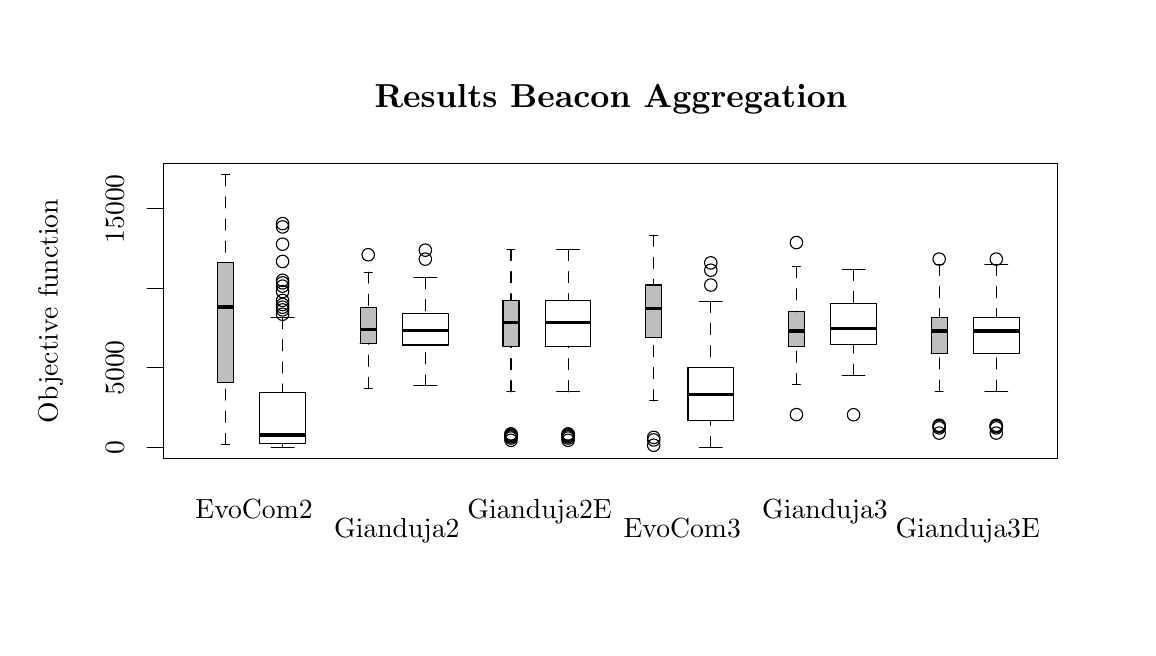
\begin{tikzpicture}[x=1pt,y=1pt]
\definecolor{fillColor}{RGB}{255,255,255}
\path[use as bounding box,fill=fillColor,fill opacity=0.00] (0,0) rectangle (397.48,216.81);
\begin{scope}
\path[clip] ( 49.20, 61.20) rectangle (372.28,167.61);
\definecolor{fillColor}{RGB}{190,190,190}

\path[fill=fillColor] ( 68.59, 88.69) --
	( 74.37, 88.69) --
	( 74.37,131.87) --
	( 68.59,131.87) --
	cycle;
\definecolor{drawColor}{RGB}{0,0,0}

\path[draw=drawColor,line width= 1.2pt,line join=round] ( 68.59,115.91) -- ( 74.37,115.91);

\path[draw=drawColor,line width= 0.4pt,dash pattern=on 4pt off 4pt ,line join=round,line cap=round] ( 71.48, 66.23) -- ( 71.48, 88.69);

\path[draw=drawColor,line width= 0.4pt,dash pattern=on 4pt off 4pt ,line join=round,line cap=round] ( 71.48,163.67) -- ( 71.48,131.87);

\path[draw=drawColor,line width= 0.4pt,line join=round,line cap=round] ( 70.04, 66.23) -- ( 72.93, 66.23);

\path[draw=drawColor,line width= 0.4pt,line join=round,line cap=round] ( 70.04,163.67) -- ( 72.93,163.67);

\path[draw=drawColor,line width= 0.4pt,line join=round,line cap=round] ( 68.59, 88.69) --
	( 74.37, 88.69) --
	( 74.37,131.87) --
	( 68.59,131.87) --
	( 68.59, 88.69);
\definecolor{fillColor}{RGB}{255,255,255}

\path[fill=fillColor] ( 83.86, 66.60) --
	(100.37, 66.60) --
	(100.37, 85.11) --
	( 83.86, 85.11) --
	cycle;

\path[draw=drawColor,line width= 1.2pt,line join=round] ( 83.86, 69.60) -- (100.37, 69.60);

\path[draw=drawColor,line width= 0.4pt,dash pattern=on 4pt off 4pt ,line join=round,line cap=round] ( 92.11, 65.14) -- ( 92.11, 66.60);

\path[draw=drawColor,line width= 0.4pt,dash pattern=on 4pt off 4pt ,line join=round,line cap=round] ( 92.11,112.04) -- ( 92.11, 85.11);

\path[draw=drawColor,line width= 0.4pt,line join=round,line cap=round] ( 87.99, 65.14) -- ( 96.24, 65.14);

\path[draw=drawColor,line width= 0.4pt,line join=round,line cap=round] ( 87.99,112.04) -- ( 96.24,112.04);

\path[draw=drawColor,line width= 0.4pt,line join=round,line cap=round] ( 83.86, 66.60) --
	(100.37, 66.60) --
	(100.37, 85.11) --
	( 83.86, 85.11) --
	( 83.86, 66.60);

\path[draw=drawColor,line width= 0.4pt,line join=round,line cap=round] ( 92.11,114.83) circle (  2.25);

\path[draw=drawColor,line width= 0.4pt,line join=round,line cap=round] ( 92.11,118.25) circle (  2.25);

\path[draw=drawColor,line width= 0.4pt,line join=round,line cap=round] ( 92.11,125.54) circle (  2.25);

\path[draw=drawColor,line width= 0.4pt,line join=round,line cap=round] ( 92.11,116.76) circle (  2.25);

\path[draw=drawColor,line width= 0.4pt,line join=round,line cap=round] ( 92.11,144.80) circle (  2.25);

\path[draw=drawColor,line width= 0.4pt,line join=round,line cap=round] ( 92.11,138.57) circle (  2.25);

\path[draw=drawColor,line width= 0.4pt,line join=round,line cap=round] ( 92.11,121.44) circle (  2.25);

\path[draw=drawColor,line width= 0.4pt,line join=round,line cap=round] ( 92.11,113.25) circle (  2.25);

\path[draw=drawColor,line width= 0.4pt,line join=round,line cap=round] ( 92.11,132.33) circle (  2.25);

\path[draw=drawColor,line width= 0.4pt,line join=round,line cap=round] ( 92.11,124.60) circle (  2.25);

\path[draw=drawColor,line width= 0.4pt,line join=round,line cap=round] ( 92.11,146.02) circle (  2.25);

\path[draw=drawColor,line width= 0.4pt,line join=round,line cap=round] ( 92.11,123.40) circle (  2.25);

\path[draw=drawColor,line width= 0.4pt,line join=round,line cap=round] ( 92.11,115.80) circle (  2.25);
\definecolor{fillColor}{RGB}{190,190,190}

\path[fill=fillColor] (120.17,102.82) --
	(125.95,102.82) --
	(125.95,115.59) --
	(120.17,115.59) --
	cycle;

\path[draw=drawColor,line width= 1.2pt,line join=round] (120.17,107.79) -- (125.95,107.79);

\path[draw=drawColor,line width= 0.4pt,dash pattern=on 4pt off 4pt ,line join=round,line cap=round] (123.06, 86.43) -- (123.06,102.82);

\path[draw=drawColor,line width= 0.4pt,dash pattern=on 4pt off 4pt ,line join=round,line cap=round] (123.06,128.49) -- (123.06,115.59);

\path[draw=drawColor,line width= 0.4pt,line join=round,line cap=round] (121.62, 86.43) -- (124.50, 86.43);

\path[draw=drawColor,line width= 0.4pt,line join=round,line cap=round] (121.62,128.49) -- (124.50,128.49);

\path[draw=drawColor,line width= 0.4pt,line join=round,line cap=round] (120.17,102.82) --
	(125.95,102.82) --
	(125.95,115.59) --
	(120.17,115.59) --
	(120.17,102.82);

\path[draw=drawColor,line width= 0.4pt,line join=round,line cap=round] (123.06,134.75) circle (  2.25);
\definecolor{fillColor}{RGB}{255,255,255}

\path[fill=fillColor] (135.44,102.15) --
	(151.94,102.15) --
	(151.94,113.51) --
	(135.44,113.51) --
	cycle;

\path[draw=drawColor,line width= 1.2pt,line join=round] (135.44,107.50) -- (151.94,107.50);

\path[draw=drawColor,line width= 0.4pt,dash pattern=on 4pt off 4pt ,line join=round,line cap=round] (143.69, 87.36) -- (143.69,102.15);

\path[draw=drawColor,line width= 0.4pt,dash pattern=on 4pt off 4pt ,line join=round,line cap=round] (143.69,126.49) -- (143.69,113.51);

\path[draw=drawColor,line width= 0.4pt,line join=round,line cap=round] (139.56, 87.36) -- (147.82, 87.36);

\path[draw=drawColor,line width= 0.4pt,line join=round,line cap=round] (139.56,126.49) -- (147.82,126.49);

\path[draw=drawColor,line width= 0.4pt,line join=round,line cap=round] (135.44,102.15) --
	(151.94,102.15) --
	(151.94,113.51) --
	(135.44,113.51) --
	(135.44,102.15);

\path[draw=drawColor,line width= 0.4pt,line join=round,line cap=round] (143.69,133.17) circle (  2.25);

\path[draw=drawColor,line width= 0.4pt,line join=round,line cap=round] (143.69,136.41) circle (  2.25);
\definecolor{fillColor}{RGB}{190,190,190}

\path[fill=fillColor] (171.75,101.72) --
	(177.53,101.72) --
	(177.53,118.31) --
	(171.75,118.31) --
	cycle;

\path[draw=drawColor,line width= 1.2pt,line join=round] (171.75,110.28) -- (177.53,110.28);

\path[draw=drawColor,line width= 0.4pt,dash pattern=on 4pt off 4pt ,line join=round,line cap=round] (174.64, 85.22) -- (174.64,101.72);

\path[draw=drawColor,line width= 0.4pt,dash pattern=on 4pt off 4pt ,line join=round,line cap=round] (174.64,136.66) -- (174.64,118.31);

\path[draw=drawColor,line width= 0.4pt,line join=round,line cap=round] (173.19, 85.22) -- (176.08, 85.22);

\path[draw=drawColor,line width= 0.4pt,line join=round,line cap=round] (173.19,136.66) -- (176.08,136.66);

\path[draw=drawColor,line width= 0.4pt,line join=round,line cap=round] (171.75,101.72) --
	(177.53,101.72) --
	(177.53,118.31) --
	(171.75,118.31) --
	(171.75,101.72);

\path[draw=drawColor,line width= 0.4pt,line join=round,line cap=round] (174.64, 68.52) circle (  2.25);

\path[draw=drawColor,line width= 0.4pt,line join=round,line cap=round] (174.64, 70.01) circle (  2.25);

\path[draw=drawColor,line width= 0.4pt,line join=round,line cap=round] (174.64, 69.25) circle (  2.25);

\path[draw=drawColor,line width= 0.4pt,line join=round,line cap=round] (174.64, 69.51) circle (  2.25);

\path[draw=drawColor,line width= 0.4pt,line join=round,line cap=round] (174.64, 67.71) circle (  2.25);

\path[draw=drawColor,line width= 0.4pt,line join=round,line cap=round] (174.64, 68.93) circle (  2.25);

\path[draw=drawColor,line width= 0.4pt,line join=round,line cap=round] (174.64, 69.91) circle (  2.25);
\definecolor{fillColor}{RGB}{255,255,255}

\path[fill=fillColor] (187.02,101.72) --
	(203.52,101.72) --
	(203.52,118.31) --
	(187.02,118.31) --
	cycle;

\path[draw=drawColor,line width= 1.2pt,line join=round] (187.02,110.28) -- (203.52,110.28);

\path[draw=drawColor,line width= 0.4pt,dash pattern=on 4pt off 4pt ,line join=round,line cap=round] (195.27, 85.22) -- (195.27,101.72);

\path[draw=drawColor,line width= 0.4pt,dash pattern=on 4pt off 4pt ,line join=round,line cap=round] (195.27,136.66) -- (195.27,118.31);

\path[draw=drawColor,line width= 0.4pt,line join=round,line cap=round] (191.14, 85.22) -- (199.40, 85.22);

\path[draw=drawColor,line width= 0.4pt,line join=round,line cap=round] (191.14,136.66) -- (199.40,136.66);

\path[draw=drawColor,line width= 0.4pt,line join=round,line cap=round] (187.02,101.72) --
	(203.52,101.72) --
	(203.52,118.31) --
	(187.02,118.31) --
	(187.02,101.72);

\path[draw=drawColor,line width= 0.4pt,line join=round,line cap=round] (195.27, 68.52) circle (  2.25);

\path[draw=drawColor,line width= 0.4pt,line join=round,line cap=round] (195.27, 70.01) circle (  2.25);

\path[draw=drawColor,line width= 0.4pt,line join=round,line cap=round] (195.27, 69.25) circle (  2.25);

\path[draw=drawColor,line width= 0.4pt,line join=round,line cap=round] (195.27, 69.51) circle (  2.25);

\path[draw=drawColor,line width= 0.4pt,line join=round,line cap=round] (195.27, 67.71) circle (  2.25);

\path[draw=drawColor,line width= 0.4pt,line join=round,line cap=round] (195.27, 68.93) circle (  2.25);

\path[draw=drawColor,line width= 0.4pt,line join=round,line cap=round] (195.27, 69.91) circle (  2.25);
\definecolor{fillColor}{RGB}{190,190,190}

\path[fill=fillColor] (223.33,104.71) --
	(229.10,104.71) --
	(229.10,123.84) --
	(223.33,123.84) --
	cycle;

\path[draw=drawColor,line width= 1.2pt,line join=round] (223.33,115.25) -- (229.10,115.25);

\path[draw=drawColor,line width= 0.4pt,dash pattern=on 4pt off 4pt ,line join=round,line cap=round] (226.22, 81.99) -- (226.22,104.71);

\path[draw=drawColor,line width= 0.4pt,dash pattern=on 4pt off 4pt ,line join=round,line cap=round] (226.22,141.82) -- (226.22,123.84);

\path[draw=drawColor,line width= 0.4pt,line join=round,line cap=round] (224.77, 81.99) -- (227.66, 81.99);

\path[draw=drawColor,line width= 0.4pt,line join=round,line cap=round] (224.77,141.82) -- (227.66,141.82);

\path[draw=drawColor,line width= 0.4pt,line join=round,line cap=round] (223.33,104.71) --
	(229.10,104.71) --
	(229.10,123.84) --
	(223.33,123.84) --
	(223.33,104.71);

\path[draw=drawColor,line width= 0.4pt,line join=round,line cap=round] (226.22, 68.76) circle (  2.25);

\path[draw=drawColor,line width= 0.4pt,line join=round,line cap=round] (226.22, 67.84) circle (  2.25);

\path[draw=drawColor,line width= 0.4pt,line join=round,line cap=round] (226.22, 65.92) circle (  2.25);
\definecolor{fillColor}{RGB}{255,255,255}

\path[fill=fillColor] (238.59, 74.76) --
	(255.10, 74.76) --
	(255.10, 94.10) --
	(238.59, 94.10) --
	cycle;

\path[draw=drawColor,line width= 1.2pt,line join=round] (238.59, 84.31) -- (255.10, 84.31);

\path[draw=drawColor,line width= 0.4pt,dash pattern=on 4pt off 4pt ,line join=round,line cap=round] (246.85, 65.14) -- (246.85, 74.76);

\path[draw=drawColor,line width= 0.4pt,dash pattern=on 4pt off 4pt ,line join=round,line cap=round] (246.85,117.91) -- (246.85, 94.10);

\path[draw=drawColor,line width= 0.4pt,line join=round,line cap=round] (242.72, 65.14) -- (250.97, 65.14);

\path[draw=drawColor,line width= 0.4pt,line join=round,line cap=round] (242.72,117.91) -- (250.97,117.91);

\path[draw=drawColor,line width= 0.4pt,line join=round,line cap=round] (238.59, 74.76) --
	(255.10, 74.76) --
	(255.10, 94.10) --
	(238.59, 94.10) --
	(238.59, 74.76);

\path[draw=drawColor,line width= 0.4pt,line join=round,line cap=round] (246.85,131.83) circle (  2.25);

\path[draw=drawColor,line width= 0.4pt,line join=round,line cap=round] (246.85,129.17) circle (  2.25);

\path[draw=drawColor,line width= 0.4pt,line join=round,line cap=round] (246.85,123.81) circle (  2.25);
\definecolor{fillColor}{RGB}{190,190,190}

\path[fill=fillColor] (274.91,101.52) --
	(280.68,101.52) --
	(280.68,114.12) --
	(274.91,114.12) --
	cycle;

\path[draw=drawColor,line width= 1.2pt,line join=round] (274.91,107.16) -- (280.68,107.16);

\path[draw=drawColor,line width= 0.4pt,dash pattern=on 4pt off 4pt ,line join=round,line cap=round] (277.79, 87.90) -- (277.79,101.52);

\path[draw=drawColor,line width= 0.4pt,dash pattern=on 4pt off 4pt ,line join=round,line cap=round] (277.79,130.42) -- (277.79,114.12);

\path[draw=drawColor,line width= 0.4pt,line join=round,line cap=round] (276.35, 87.90) -- (279.24, 87.90);

\path[draw=drawColor,line width= 0.4pt,line join=round,line cap=round] (276.35,130.42) -- (279.24,130.42);

\path[draw=drawColor,line width= 0.4pt,line join=round,line cap=round] (274.91,101.52) --
	(280.68,101.52) --
	(280.68,114.12) --
	(274.91,114.12) --
	(274.91,101.52);

\path[draw=drawColor,line width= 0.4pt,line join=round,line cap=round] (277.79, 76.99) circle (  2.25);

\path[draw=drawColor,line width= 0.4pt,line join=round,line cap=round] (277.79,139.16) circle (  2.25);
\definecolor{fillColor}{RGB}{255,255,255}

\path[fill=fillColor] (290.17,102.31) --
	(306.68,102.31) --
	(306.68,117.26) --
	(290.17,117.26) --
	cycle;

\path[draw=drawColor,line width= 1.2pt,line join=round] (290.17,108.02) -- (306.68,108.02);

\path[draw=drawColor,line width= 0.4pt,dash pattern=on 4pt off 4pt ,line join=round,line cap=round] (298.43, 91.21) -- (298.43,102.31);

\path[draw=drawColor,line width= 0.4pt,dash pattern=on 4pt off 4pt ,line join=round,line cap=round] (298.43,129.54) -- (298.43,117.26);

\path[draw=drawColor,line width= 0.4pt,line join=round,line cap=round] (294.30, 91.21) -- (302.55, 91.21);

\path[draw=drawColor,line width= 0.4pt,line join=round,line cap=round] (294.30,129.54) -- (302.55,129.54);

\path[draw=drawColor,line width= 0.4pt,line join=round,line cap=round] (290.17,102.31) --
	(306.68,102.31) --
	(306.68,117.26) --
	(290.17,117.26) --
	(290.17,102.31);

\path[draw=drawColor,line width= 0.4pt,line join=round,line cap=round] (298.43, 76.94) circle (  2.25);
\definecolor{fillColor}{RGB}{190,190,190}

\path[fill=fillColor] (326.48, 99.09) --
	(332.26, 99.09) --
	(332.26,112.18) --
	(326.48,112.18) --
	cycle;

\path[draw=drawColor,line width= 1.2pt,line join=round] (326.48,107.15) -- (332.26,107.15);

\path[draw=drawColor,line width= 0.4pt,dash pattern=on 4pt off 4pt ,line join=round,line cap=round] (329.37, 85.48) -- (329.37, 99.09);

\path[draw=drawColor,line width= 0.4pt,dash pattern=on 4pt off 4pt ,line join=round,line cap=round] (329.37,131.27) -- (329.37,112.18);

\path[draw=drawColor,line width= 0.4pt,line join=round,line cap=round] (327.93, 85.48) -- (330.82, 85.48);

\path[draw=drawColor,line width= 0.4pt,line join=round,line cap=round] (327.93,131.27) -- (330.82,131.27);

\path[draw=drawColor,line width= 0.4pt,line join=round,line cap=round] (326.48, 99.09) --
	(332.26, 99.09) --
	(332.26,112.18) --
	(326.48,112.18) --
	(326.48, 99.09);

\path[draw=drawColor,line width= 0.4pt,line join=round,line cap=round] (329.37, 72.19) circle (  2.25);

\path[draw=drawColor,line width= 0.4pt,line join=round,line cap=round] (329.37, 72.84) circle (  2.25);

\path[draw=drawColor,line width= 0.4pt,line join=round,line cap=round] (329.37, 70.31) circle (  2.25);

\path[draw=drawColor,line width= 0.4pt,line join=round,line cap=round] (329.37, 72.72) circle (  2.25);

\path[draw=drawColor,line width= 0.4pt,line join=round,line cap=round] (329.37, 73.15) circle (  2.25);

\path[draw=drawColor,line width= 0.4pt,line join=round,line cap=round] (329.37,133.19) circle (  2.25);
\definecolor{fillColor}{RGB}{255,255,255}

\path[fill=fillColor] (341.75, 99.09) --
	(358.26, 99.09) --
	(358.26,112.18) --
	(341.75,112.18) --
	cycle;

\path[draw=drawColor,line width= 1.2pt,line join=round] (341.75,107.15) -- (358.26,107.15);

\path[draw=drawColor,line width= 0.4pt,dash pattern=on 4pt off 4pt ,line join=round,line cap=round] (350.00, 85.48) -- (350.00, 99.09);

\path[draw=drawColor,line width= 0.4pt,dash pattern=on 4pt off 4pt ,line join=round,line cap=round] (350.00,131.27) -- (350.00,112.18);

\path[draw=drawColor,line width= 0.4pt,line join=round,line cap=round] (345.88, 85.48) -- (354.13, 85.48);

\path[draw=drawColor,line width= 0.4pt,line join=round,line cap=round] (345.88,131.27) -- (354.13,131.27);

\path[draw=drawColor,line width= 0.4pt,line join=round,line cap=round] (341.75, 99.09) --
	(358.26, 99.09) --
	(358.26,112.18) --
	(341.75,112.18) --
	(341.75, 99.09);

\path[draw=drawColor,line width= 0.4pt,line join=round,line cap=round] (350.00, 72.19) circle (  2.25);

\path[draw=drawColor,line width= 0.4pt,line join=round,line cap=round] (350.00, 72.84) circle (  2.25);

\path[draw=drawColor,line width= 0.4pt,line join=round,line cap=round] (350.00, 70.31) circle (  2.25);

\path[draw=drawColor,line width= 0.4pt,line join=round,line cap=round] (350.00, 72.72) circle (  2.25);

\path[draw=drawColor,line width= 0.4pt,line join=round,line cap=round] (350.00, 73.15) circle (  2.25);

\path[draw=drawColor,line width= 0.4pt,line join=round,line cap=round] (350.00,133.19) circle (  2.25);
\end{scope}
\begin{scope}
\path[clip] (  0.00,  0.00) rectangle (397.48,216.81);
\definecolor{drawColor}{RGB}{0,0,0}

\node[text=drawColor,rotate= 90.00,anchor=base,inner sep=0pt, outer sep=0pt, scale=  1.00] at ( 10.80,114.41) {Objective function};
\end{scope}
\begin{scope}
\path[clip] (  0.00,  0.00) rectangle (397.48,216.81);
\definecolor{drawColor}{RGB}{0,0,0}

\node[text=drawColor,anchor=base,inner sep=0pt, outer sep=0pt, scale=  1.00] at ( 81.80, 39.60) {EvoCom2};

\node[text=drawColor,anchor=base,inner sep=0pt, outer sep=0pt, scale=  1.00] at (184.95, 39.60) {Gianduja2E};

\node[text=drawColor,anchor=base,inner sep=0pt, outer sep=0pt, scale=  1.00] at (288.11, 39.60) {Gianduja3};

\node[text=drawColor,anchor=base,inner sep=0pt, outer sep=0pt, scale=  1.00] at (133.38, 32.71) {Gianduja2};

\node[text=drawColor,anchor=base,inner sep=0pt, outer sep=0pt, scale=  1.00] at (236.53, 32.71) {EvoCom3};

\node[text=drawColor,anchor=base,inner sep=0pt, outer sep=0pt, scale=  1.00] at (339.69, 32.71) {Gianduja3E};
\end{scope}
\begin{scope}
\path[clip] (  0.00,  0.00) rectangle (397.48,216.81);
\definecolor{drawColor}{RGB}{0,0,0}

\node[text=drawColor,anchor=base,inner sep=0pt, outer sep=0pt, scale=  1.20] at (210.74,188.07) {\bfseries Results Beacon Aggregation};
\end{scope}
\begin{scope}
\path[clip] (  0.00,  0.00) rectangle (397.48,216.81);
\definecolor{drawColor}{RGB}{0,0,0}

\path[draw=drawColor,line width= 0.4pt,line join=round,line cap=round] ( 49.20, 65.14) -- ( 49.20,151.36);

\path[draw=drawColor,line width= 0.4pt,line join=round,line cap=round] ( 49.20, 65.14) -- ( 43.20, 65.14);

\path[draw=drawColor,line width= 0.4pt,line join=round,line cap=round] ( 49.20, 93.88) -- ( 43.20, 93.88);

\path[draw=drawColor,line width= 0.4pt,line join=round,line cap=round] ( 49.20,122.62) -- ( 43.20,122.62);

\path[draw=drawColor,line width= 0.4pt,line join=round,line cap=round] ( 49.20,151.36) -- ( 43.20,151.36);

\node[text=drawColor,rotate= 90.00,anchor=base,inner sep=0pt, outer sep=0pt, scale=  1.00] at ( 34.80, 65.14) {0};

\node[text=drawColor,rotate= 90.00,anchor=base,inner sep=0pt, outer sep=0pt, scale=  1.00] at ( 34.80, 93.88) {5000};

\node[text=drawColor,rotate= 90.00,anchor=base,inner sep=0pt, outer sep=0pt, scale=  1.00] at ( 34.80,151.36) {15000};

\path[draw=drawColor,line width= 0.4pt,line join=round,line cap=round] ( 49.20, 61.20) --
	(372.28, 61.20) --
	(372.28,167.61) --
	( 49.20,167.61) --
	( 49.20, 61.20);
\end{scope}
\end{tikzpicture}
